\section{Bemeneti és kimeneti paraméterek}
\subsection{Szövegfüggő címkék}
A címke generálás egységeként egy mondatot használtunk fel. Ezt az NLTK eszköz segítségével elemeztük majd az eredményekből állítottuk össze a címkéket[6]. A címkék alapjául az aktuális fonémák szolgáltak, később még ezek lettek továbbontva időkeret szerint.A fonéma azonosítására OneHot kódolást alkalmaztunk, azaz minden fonémát 40 értékkel azonosítottunk.

A következő szöveg függő címkéket hoztuk létre:

\begin{itemize}
	\item 1-5 aktuális fonéma és az őt körülvevő két-két fonéma
	\item 6 hangsúly
	\item 7-8 megelőző és követő fonémák száma a szóban 
	\item 9-10 távolság hangsúlyos fonémától mindkét irányban
	\item 11 szó szófaja
	\item 12-13 szó pozíciója a mondatban
	\item 14-16 fonémák száma az aktuális szóban és két szomszédjában
	\item 17 szavak száma a mondatban
	\item 18 fonémák száma a mondatban
\end{itemize}

\subsection{Bemeneti paraméterek}
A szövegfüggő fonéma címkéket egészítettük ki a fonémában található időkeretek számával és a keret fonémán belüli elhelyezkedésével. Így a kerethez tartozó 215 bemeneti paraméter az alábbiakból tevődik össze:

\begin{itemize}
	\item 1-200 A 40-40 paraméter a kvinfón(2-1-2) fonémáira
	\item 201-213 további szövegfüggő címkék
	\item 214 A fonémán belüli időkeretek száma
	\item 215 A keret elhelyezkedése a fonémán belül
\end{itemize} 
\begin{figure}[h]
	\par\centering
	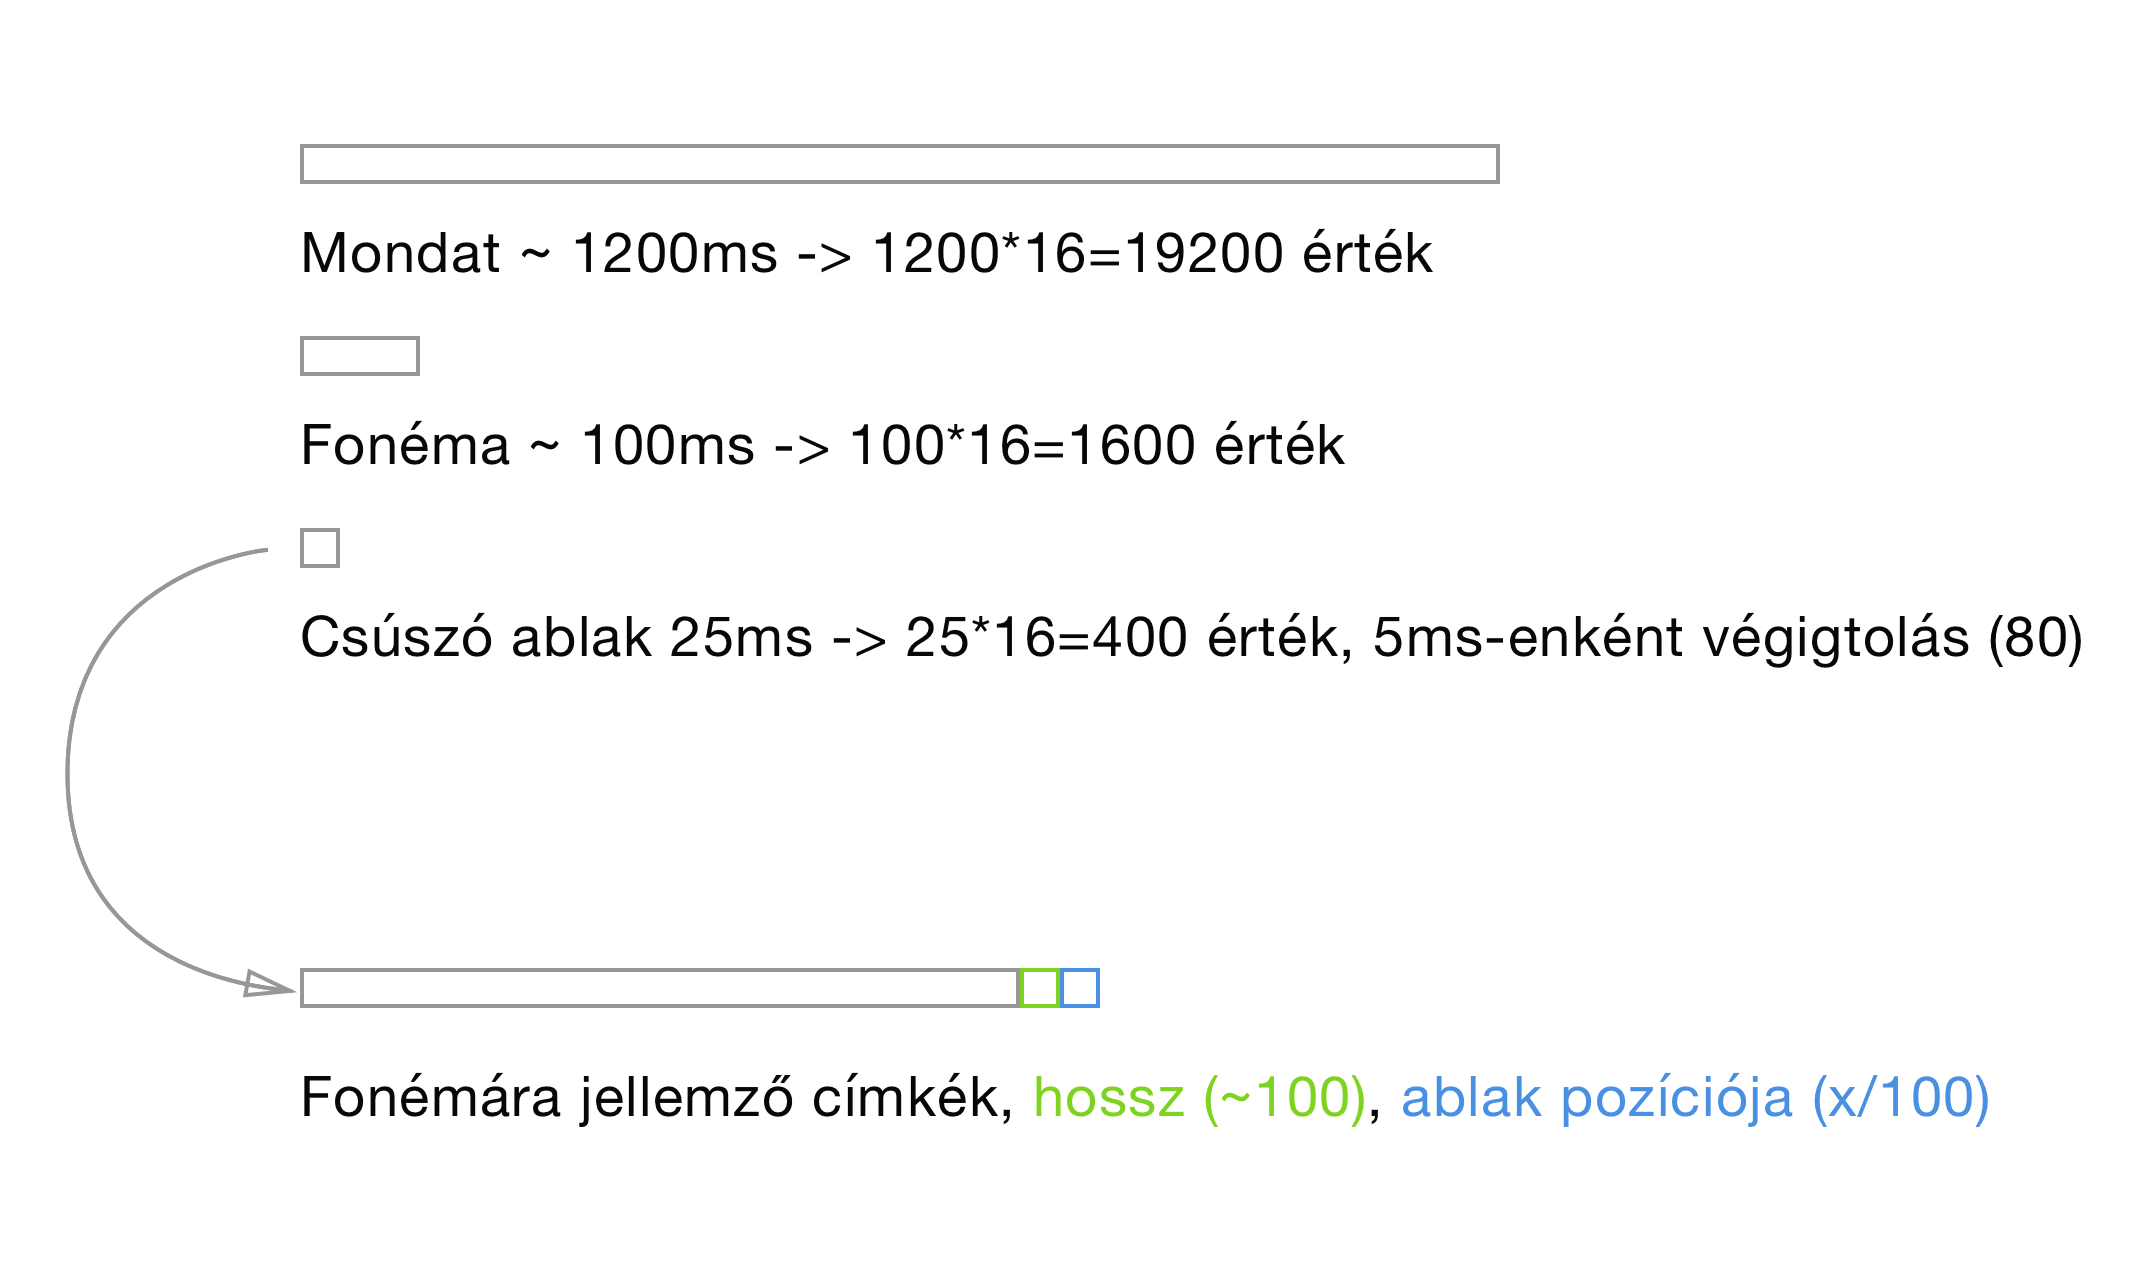
\includegraphics[width=0.8\textwidth,keepaspectratio]{tag_struct}
	\caption{Címkék létrehozásának folyamata}
\end{figure}

\subsection{Kimeneti paraméterek}
Az előző felsorolást folytatva az aktuális időkerethez tartozó elvárt kimenet paraméterek a következők:

 
\begin{itemize}
	\item 215 a keret hangmagasság értéke
	\item 216-242 a Mel-Cepstrum 26 paramétere
	\item 242 a fonémán belüli keretek száma
\end{itemize}
\subsection{Spektrális és gerjesztési paraméterek}
Mint említettük a prediktálás alapja a spektrális és gerjesztési paraméterek megadása keretenként. Ezen paraméterek segítségével a PyPSTK
\footnote{http://pysptk.readthedocs.io/}
python csomag használatával állíthatjuk elő az audio kimenetet, valamint hasonlóképpen ezt a csomagot használjuk az adataink a tiszta hangból való előállítására \ [2].
\subsubsection{Mel-Cepstrum}
A paraméterek előállításához, visszafejtéséhez a PyPSTK Mel-Cepstrum alapú algoritmusát alkalmazzuk. Az algoritmust T. Fukada és társai fejlesztették ki.\ [3]


Ezzel a metódussal természetesen adatvesztést kapunk, azonban az így előállított hang még megfelel a mércéinknek. Viszont az általunk generált kimenetek értékelésénél ezt figyelembe kell vennünk.
\begin{figure}[h]
	\par
	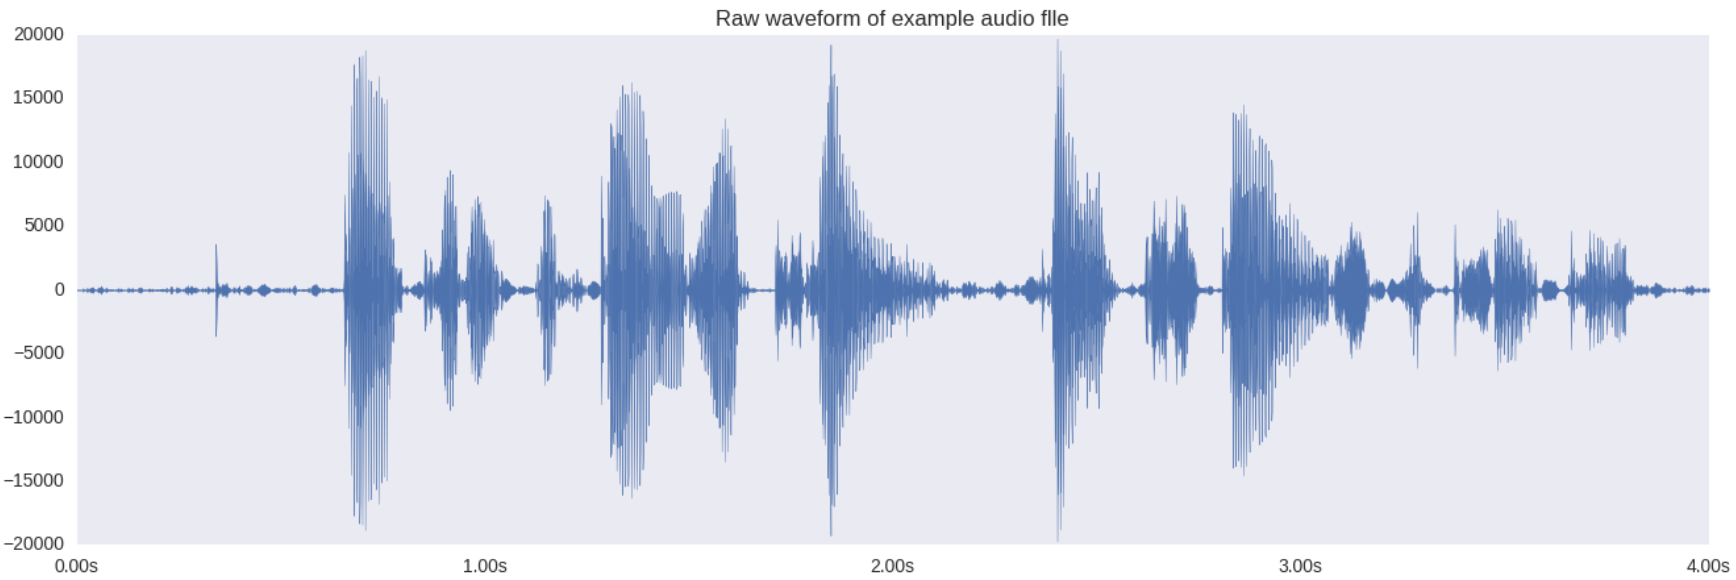
\includegraphics[width=\textwidth,keepaspectratio]{audio_raw}
	\caption{Eredeti hang}
\end{figure}
\begin{figure}[h]
	\par
	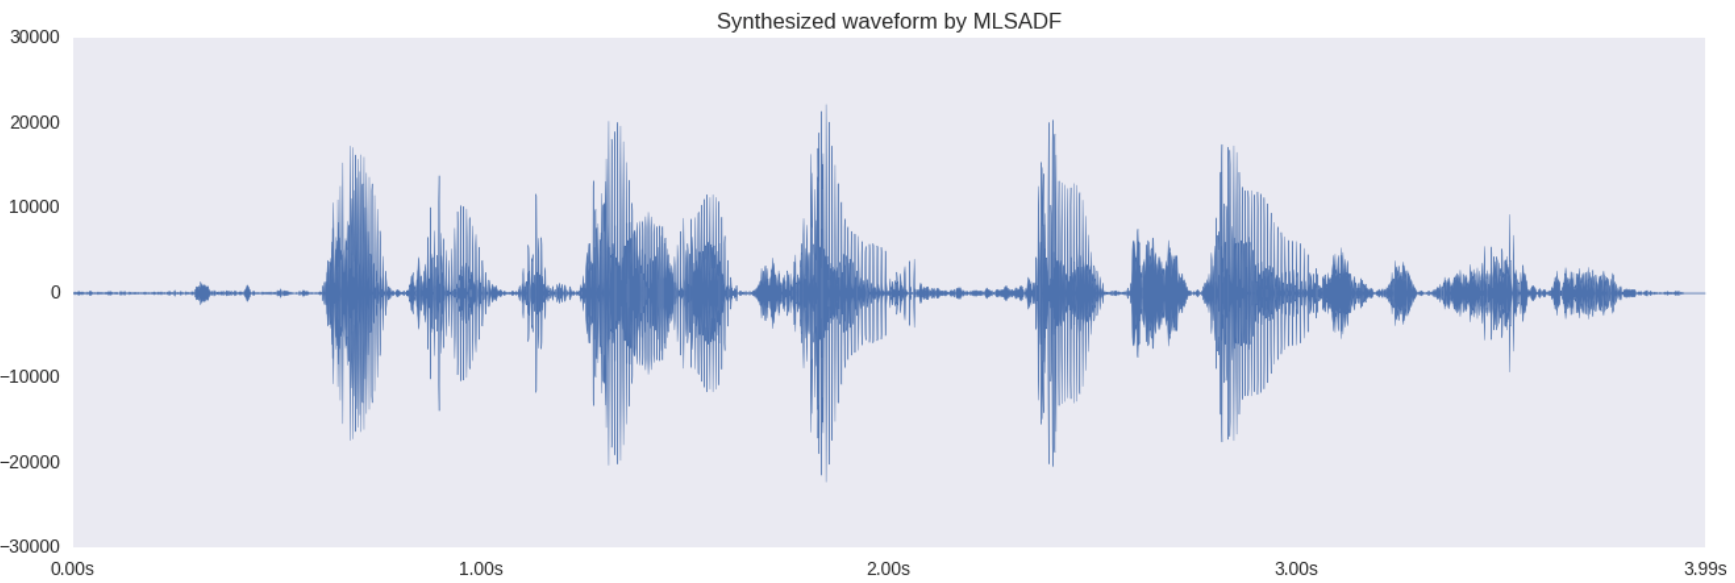
\includegraphics[width=\textwidth,keepaspectratio]{audio_mc}
	\caption{Mel-Cepstrum után elállítható hang}
\end{figure}
